
\documentclass{article}
\usepackage[utf8]{inputenc}
\usepackage[normalem]{ulem}
\usepackage{listings}
\usepackage{hyperref}

\hypersetup{
    colorlinks=true,
    linkcolor=red,
    filecolor=magenta,      
    urlcolor=cyan,
}
\usepackage{graphicx}
\usepackage{amsmath}
\usepackage{amsfonts}
\usepackage{amssymb}
\usepackage{array}
\usepackage{float}
\restylefloat{table}
%fancy headers
\usepackage{fancyhdr}
\pagestyle{fancy}
\fancyhf{}
\lhead{ICSI 401 Homework 4}
\rhead{\thepage}
\author{James Oswald}
\date{November 18, 2020}
\title{ICSI 401 Homework 4}

\begin{document}
\maketitle
\thispagestyle{fancy}
\addtocounter{section}{4}
\subsection{Partial pivoting}
In this problem, you will review partial pivoting and the reasoning behind it.
\begin{itemize}
    \item[1.]  Circle the best explanation for the use of partial pivoting from the choices below.
    \begin{itemize}
        \item[(a)] Partial pivoting is used in Gaussian elimination to mitigate the effects of rounding errors in the matrix entries, resulting in an algorithm that is usually backward stable.
        \item[(b)] Partial pivoting is not used in Gaussian elimination at all, but is instead used to solve linear systems via Cramer’s rule.
        \item[(c)] Partial pivoting is used to transform the input to Gaussian elimination so as to speed up the solution of linear systems.
    \end{itemize}
    \noindent
    \newline\newline\newline
    The correct answer is choice A: Partial pivoting is used in Gaussian elimination to mitigate the effects of rounding errors in the matrix entries, resulting in an algorithm that is usually backward stable.
    
    \newpage
    \item[2.] . Show the steps of Gaussian elimination with partial pivoting for the following matrix:
    \[\begin{pmatrix} 10^{-5} & 1 & 0 \\ 2 & -3 & 1 \\ -1 & 1 & 1 \end{pmatrix}\]
    Make sure that you clearly indicate in each step what operation you are performing (e.g., which rows are swapped, which multiples of rows are added to which other rows) and the result of that operation. You should end up with an upper triangular matrix.
    \begin{align*}
        \begin{pmatrix} 0.00001 & 1 & 0 \\ 2 & -3 & 1 \\ -1 & 1 & 1 \end{pmatrix}
        & R_2\leftrightarrow R_1 & \text{Pivot element is 2}\\
        \begin{pmatrix} 2 & -3 & 1 \\ 0.00001 & 1 & 0 \\ -1 & 1 & 1 \end{pmatrix}
        & \frac{1}{2}R_1\rightarrow R_1 &\\
        \begin{pmatrix} 1 & -1.5 & 0.5 \\ 0.00001 & 1 & 0 \\ -1 & 1 & 1 \end{pmatrix}
        & R_2 + (-0.0001)R_1\rightarrow R_2 &\\
        \begin{pmatrix} 1 & -1.5 & 0.5 \\ 0 & 1.000015 & 1.000005 \\ -1 & 1 & 1 \end{pmatrix}
        & R_3 + R_1\rightarrow R_3 &\\
        \begin{pmatrix} 1 & -1.5 & 0.5 \\ 0 & 1.000015 & 1.000005 \\ 0 & -0.5 & 1.5 \end{pmatrix}
        & \frac{1}{1.000015}R_2\rightarrow R_2 & \text{Pivot element is 1.000015} \\
        \begin{pmatrix} 1 & -1.5 & 0.5 \\ 0 & 1 & 0.000004999 \\ 0 & -0.5 & 1.5 \end{pmatrix}
        & R_3 + (0.5)R_2\rightarrow R_3 & \\
        \begin{pmatrix} 1 & -1.5 & 0.5 \\ 0 & 1 & 0.000004999 \\ 0 & 0 & 1.500002499 \end{pmatrix}
        & \frac{1}{1.500002499}R_3\rightarrow R_3 \\
        \begin{pmatrix} 1 & -1.5 & 0.5 \\ 0 & 1 & 0.000004999 \\ 0 & 0 & 1 \end{pmatrix}
    \end{align*}
\end{itemize}

\newpage
\subsection{Least squares and curve fitting}
This problem will give you practice in using least squares to fit polynomials to data. Consider the following dataset in Matlab, consisting of pairs of points $(x, y)$:
\begin{verbatim}
    x = [-3, -2, -1, 0, 1, 2, 3]’;
    y = [-12.529999999999999, -3.02, 0.49, 1.00, 1.51, 5.02, 14.529999999999999]’;
\end{verbatim}
Suppose that you want to find a least squares fit of a degree-3 polynomial to this data. I.e., you want to determine coefficients $c0$, $c1$, $c2$, $c3$ such that $c_3x^3 + c_2x^2 + c1x + c0$ is a least-squares fit to the data. We will collect the coefficients into a vector $\overrightarrow{c_*} = [c0, c1, c2, c3]^T$.
\begin{itemize}
    \item[1.] Using Matlab, compute the Vandermonde matrix A associated with this problem and explain how you got it. Remember that least squares requires us to solve
    \[\overrightarrow{c_*} = \text{argmin}_{\overrightarrow{c}}\left\Vert A\overrightarrow{c}-\overrightarrow{y}\right\Vert^2_2\]
    \newline\newline
    I begin by computing the Vandermonde matrix of x using the format laid out by the textbook as my guideline for its construction. 
    \begin{verbatim}
        disp("The Vandermonde matrix of the problem:");
        A = [ones(size(x)) x x.^2 x.^3];
        disp(A);
    \end{verbatim}
    I run and obtain:
    \begin{verbatim}
        The Vandermonde matrix of the problem:
             1    -3     9   -27
             1    -2     4    -8
             1    -1     1    -1
             1     0     0     0
             1     1     1     1
             1     2     4     8
             1     3     9    27
    \end{verbatim}
    
    \newpage
    \item[2.] In Matlab, use the $A$ that you computed and the normal equations approach to the least squares problem to compute the vector of coefficients $\overrightarrow{c}$.
    \newline\newline
    I compute the vector of coefficients using the pseudo-inverse of $A$ and $y$.
    \begin{verbatim}
        disp("The Vector of coefficients:");
        c = pinv(A)*y;
        disp(c);
    \end{verbatim}
     I run and obtain:
    \begin{verbatim}
        The Vector of coefficients:
            1.0000
            0.0100
            0.0000
            0.5000
    \end{verbatim}
    To check my work I plot the degree 3 polynomial with the computed coefficients against the input data:
    \begin{verbatim}
        hold on
        scatter(x,y)
        fplot(@(x)c(4)*x.^3 + c(3)*x.^2 + c(2)*x + c(1));
        xlim([-5 5])
        ylim([-16 16])
        hold off
    \end{verbatim}
    And observe that this does indeed appear to fit the data very well:
    \newline\newline
    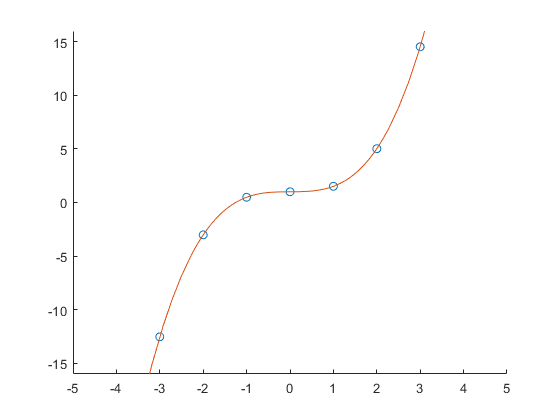
\includegraphics[scale=0.5]{Homework4/422.png}
    
    \newpage
    \item[3.] In Matlab, use the norm function to compute the the error $\left\Vert A\overrightarrow{c}-\overrightarrow{y}\right\Vert^2_2$.
    \newline\newline
    I use the norm function to help me compute the error of the degree 3 polynomial with the computed coefficients against the data. 
    \begin{verbatim}
        disp("The Error:");
        n = norm(A*c - y, 2);
        disp(n);
    \end{verbatim}
     I run and obtain a very small error:
    \begin{verbatim}
        The Error:
           2.8571e-15
    \end{verbatim}
\end{itemize}

All of my code for this problem can be found in the attached MATLAB file under the name: hw42.m

\newpage
\subsection{Eigenthings and the power method}
\begin{itemize}
    \item[1.] Using Matlab, use the power method to calculate unit eigenvectors corresponding to the dominant two eigenvalues of the matrix
    \[\begin{pmatrix} 6 & 2 & -1 \\ 2 & 5 & 1 \\ -1 & 1 & 4 \end{pmatrix}\]
    In particular, you should run the power method for 50 iterations. As usual, include your Matlab code and output. Clearly indicate the two eigenvectors that are your final answer.
\end{itemize}
I begin by implementing an algorithm to perform the power method calculating both the dominant eigenvalue $v$ and dominant eigenvector $x$ of a matrix $A$ for a set number of iterations. 
\begin{verbatim}
    function [x,v] = powerMethod(x0, A, itter)
        x = x0;
        for i = 1:itter
           z = A*x;
           x = z/norm(z);
           v = x'*A*x;
        end
    end
\end{verbatim}
From here I compute and print the true eigenvalues and vectors followed by the dominant eigenvalue and eigen vector calculated by 50 iterations of the power method.
\begin{verbatim}
    A = [6 2 -1; 2 5 1; -1 1 4];
    x = [1 1 1]';
    disp("Real Eigen Values and Vecs of A")
    [vi, ei] = eig(A);
    disp(ei);
    disp(vi);
    disp("Power method Eigen Values and Vecs of A")
    [e1, v1] = powerMethod(x, A, 50);
    disp(e1);
    disp(v1);
\end{verbatim}

\newpage
Finally I run my program and check and see that my dominant eigenvalue lines up.
\begin{verbatim}
    Real Eigen Values and Vecs of A
        2.2855         0         0
             0    5.1433         0
             0         0    7.5712
    
       -0.4918   -0.3472   -0.7985
        0.5962    0.5341   -0.5994
       -0.6346    0.7708    0.0557

    Power method Eigen Values and Vecs of A
        0.7985
        0.5994
       -0.0557
    
        7.5712
\end{verbatim}
I'm not entirely sure what it means by the dominant two eigenvalues and eigenvectors of the matrix. By definition a matrix can only have one dominant eigenvalue, thus I am confused by the nature of the question when it asks us to calculate two of them. It is clear that 7.5712 is the only dominant eigenvalue and only corresponds to one dominant eigenvector.  

\newpage
\subsection{Polynomial interpolation, Chebyshev points}
\begin{itemize}
    \item[1.] In general, if we are given points $(x_0, y_0), ...,(x_n, y_n)$, what is the minimum number $d$ such that a unique polynomial with degree $\leq d$ and passing through these points is guaranteed to exist?
    \newline\newline
    $n-1$. This can be seen by observing the pattern that arises when trying to create polynomials that fit to a set of points of arbitrary size. For 1 point, we need at least a horizontal line (polynomial of degree 0) to pass through it. For 2 points we need a line at a slope (polynomial of degree 1) since the points may not lay on the same horizontal line. With 3 points, they may not lie on a line at all so we need a parabola (polynomial of degree 1) which has at most a single bend that can reach over to a third point. This pattern continues for sets of points with size $n$ needing a polynomial of at least $n - 1$ to cover all of their points
    \item[2.] Let $x_0 = -1, x_1 = 1, x_2 = 2$, and let $y_0 = 1, y_1 = 2, y_2 = 3$. Write down the Lagrange interpolating polynomial that passes through the points $(x_0, y_0),(x_1, y_1),(x_2, y_2)$
    \newline\newline
    For 3 points the Lagrange Interpolating Polynomial takes the form P(x) after which we can substitute in and simplify. Note that I start my indices at 1, while the points start at 0, when plugging in I just shift down by 1. 
    \begin{align*}
        P(x) &= \frac{(x-x_2)(x-x_3)}{(x_1-x_2)(x_1-x_3)}y_1 + \frac{(x-x_1)(x-x_3)}{(x_2-x_1)(x_2-x_3)}y_2 + \frac{(x-x_1)(x-x_2)}{(x_3-x_1)(x_3-x_2)}y_3 \\
        P(x) &= \frac{(x-1)(x-2)}{(-1-1)(-1-2)}1 + \frac{(x--1)(x-2)}{(1--1)(1-2)}2+ \frac{(x--1)(x-1)}{(2--1)(2-1)}3\\
        P(x) &= \frac{x^2-3x+2}{6} + \frac{x^2-x-2}{-1}+ \frac{x^2-1}{1}\\
        P(x) &= \frac{x^2-3x+2-6x^2+6x+12+6x^2-6}{6}\\
        P(x) &= \frac{x^2+4x+8}{6}\\
        P(x) &= \frac{1}{6}x^2 +\frac{2}{3}x+\frac{4}{3} \\
    \end{align*}
    
    \newpage
    \item[3.] For the points in the previous problem, fill in the following divided difference table:
    \begin{center}
        \begin{tabular}{ |c|c|c| } 
         \hline
         $f[x_0]$ &  &  \\ 
         $f[x_1]$ & $f[x_0, x_1]$ &  \\ 
         $f[x_2]$ & $f[x_1, x_2]$ & $f[x_0, x_1, x_2]$ \\ 
         \hline
        \end{tabular}
    \end{center}
    In other words, what is expected is that you compute $f[x_0], f[x_1], f[x_0, x_1]$, etc.
    We begin by calculating our first column based off of the points provided.
    \begin{align*}
        f[x_0] = 1,  f[x_1] = 2, f[x_2] = 3
    \end{align*}
    Next we use the interpolation formula to calculate terms in the second column:
    \begin{align*}
        f[a, b] &= \frac{f[b]-f[a]}{b-a}\\
        f[x_0, x_1] &= \frac{f[x_1]-f[x_0]}{x_1 - x_0} = \frac{2-1}{1--1} = 0.5\\
        f[x_1, x_2] &= \frac{f[x_2]-f[x_1]}{x_2 - x_1} = \frac{3-2}{2-1} = 1\\
    \end{align*}
    Finally we use:
    \begin{align*}
        f[a, b, c] &= \frac{f[b, c]-f[a, b]}{c-a}\\
        f[x_0, x_1, x_2] &= \frac{f[x_1, x_2]-f[x_0, x_1]}{x_2-x_0} = \frac{1-0.5}{2--1} = \frac{1}{6}\\
    \end{align*}
    Thus our final table is:
      \begin{center}
        \begin{tabular}{ |c|c|c| } 
         \hline
         1 &  &  \\ 
         2 & 0.5 &  \\ 
         3 & 1 & 1.6666\\ 
         \hline
        \end{tabular}
    \end{center}
    \item[4.] Using the divided difference table above, write down the Newton interpolating polynomial for these points.
    \newline\newline
    To calculate our Newton interpolating polynomial we read off the points on the diagonal as coefficients and get the Newton form of the interpolating polynomial as  $1 + \frac{1}{2}(x+1) + \frac{1}{6}(x+1)(x-1)$
\end{itemize}

\newpage
\subsection{Piecewise polynomial interpolation}
Do Exercise 8.8.9 in the book (on piecewise polynomial interpolation).
\newline\newline
It follows from the conditions that since $P_1$ is linear and we know that $P(0) = 1$ and $P(1) = -1$ this means that our $P_1$ must be the strait line that connects these two points, namely $P_1(x) = -2x + 1$.
\newline\newline
Next we need to find $P_2$. Since we know that $P$ is continuous at 1 this means $P_2$s derivative at $1$ matches $P_1$s which is 2, Thus we know $P^{'}_2(1)=-2$. We also know $P_2$ is quadratic and that $P_2(1)=-1$ and $P_2(2)=0$. We can write $P_2$ in Newton form $a_0+a_1(x-1)+a_2(x-1)(x-2)$ From here we see that $a_0 = P_2(1) = -1$ and $-1 + a_1 = P_2(2) = 0$ thus $a_1 = 1$. Finally to derive $a_2$ we derive the derivative of $P_2$ as $P^{'}_2(x) = a_1+a_2(2x-3)$, we use this to see that $P^{'}_2(1) = 1 - c2 = -2$ thus $a_2=3$. Finally we multiply the completed newton form out yielding $3x^2-8x+4$.
Thus our final piecewise equation is:
\[ P(x)=\begin{cases} 
      -2x + 1 & 0\leq x \leq1 \\
      3x^2-8x+4 & 1\leq x\leq 2 \\
   \end{cases}
\]
Which we can then plot 

\end{document}